% ------------------------------------------------
% *** Section 1: Introduction ***
% ------------------------------------------------
% This section can be used for introduction or background information
\newpage
\chapter{Introduction}
\section{Getting Started}


AstraKernel begins its life in a small bootstrap routine, written in ARM assembly, 
that prepares the processor’s state before passing control to the main C kernel. 
This bootstrap code is responsible for setting up the stack pointer, clearing 
the uninitialized data section (\texttt{.bss}), and ensuring a clean environment 
for the kernel’s entry point.

Below is the initial assembly code that executes at startup: \\

\begin{lstlisting}[language={C}, caption={Initial bootstrap code for AstraKernel.}, label={lst:bootstrap}]
    .section .text
    .global _start

_start:
    // Set up the stack pointer
    LDR sp, =_estack
    BIC sp, sp, #7
    // Zero the .bss section
    LDR R0, =__bss_start   // Start address (symbol from linker script)
    LDR R1, =__bss_end     // End address (symbol from linker script)
    MOV R2, #0             // init zero-value for BSS clearing

zero_bss:
    // Check if we are done zeroing the BSS
    CMP R0, R1             // Compare current address to end
    BGE bss_done           // If done, skip zeroing
    STR R2, [R0], #4       // Store zero at [r0], increment r0 by 4
    B zero_bss

bss_done:
    // Call kernel_main function
    BL kernel_main

hang:
    // Halt if kernel_main returns (should not happen)
    B hang		// Infinite loop
\end{lstlisting}

This startup sequence is the essential first step for any kernel, ensuring the 
CPU is properly initialized and memory is in a known state before higher-level 
code takes over. Once these preparations are complete, the \texttt{kernel\_main} 
function from \texttt{kernel/kernel.c} is called, marking the transition from 
low-level assembly to the C code that forms the core of AstraKernel.

\subsection{Prerequisites}

Before you can build and run AstraKernel, please ensure you have the following 
tools installed on your system:

\begin{itemize}
  \item \textbf{ARM Cross-Compiler:}  
  A cross-compiler targeting ARM is required to build the kernel. It 
  is recommended to use \texttt{arm-none-eabi-gcc}, \texttt{arm-none-eabi-ld}, 
  and \texttt{arm-none-eabi-objcopy} for ARM926EJ-S, which is the target architecture
  for AstraKernel.
  \begin{itemize}
    \item Example installation: \texttt{arm-none-eabi-xxx} (available via package 
    managers such as \texttt{brew}, \texttt{apt}, or direct download from ARM's website).
  \end{itemize}
  
  \item \textbf{QEMU Emulator:}  
  QEMU is used to emulate the ARM VersatilePB (ARM926EJ-S) platform for kernel development and testing.
  \begin{itemize}
    \item Ensure your QEMU installation supports the \texttt{versatilepb} machine.
    \item Example installation: \texttt{qemu-system-arm} via  qemu \url{https://www.qemu.org/download/}.
  \end{itemize}

  \item \textbf{Build Tools:}  
  Standard build tools such as \texttt{make} are required to compile the kernel.
  \begin{itemize}
    \item Example installation: \texttt{make} (available via package managers 
    such as \texttt{brew}, \texttt{apt}, or direct download \url{https://www.gnu.org/software/make/#download}).
  \end{itemize}
\end{itemize}

\noindent
For best results, ensure all tools are up-to-date. Consult the official documentation 
of each tool for installation instructions on your operating system.

\begin{figure}[!ht]
  \centering
  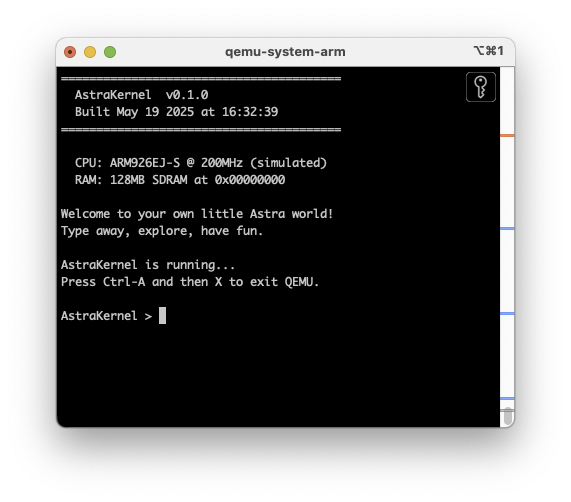
\includegraphics[width=0.6\textwidth]{figures/bootedKernel.png}
  \caption{AstraKernel booted in QEMU.}
  \label{fig:bootedKernel}
\end{figure}
